\documentclass[12pt]{article}
\usepackage{amsmath,amssymb,setspace,verbatim,graphicx,enumerate,enumitem}
\usepackage[top=.8in,bottom=.8in,left=1in,right=1in,nohead,nofoot]{geometry}
\usepackage{caption}
%\usepackage{subcaption}
\usepackage{subfig}
\usepackage{subfloat}
\usepackage{tabularx}
\parindent 0in
\parskip .2in
\pagestyle{empty} \singlespacing
%\newcommand{\vect}[1]{\mbox{\boldmath $ #1$}}
\newcommand{\bv}[1]{\mathbf{#1}}
%\setlist{noitemsep,topsep=0pt,parsep=0pt,partopsep=0pt}


\begin{document}
%
\baselineskip=15.5pt
\begin{center}
{\bf STA6320 - FDA} \\
{\bf Homework 1} \\
{\bf Seokjun Choi} \\
\end{center}
hello

\begin{itemize}
\item Chapter 1

\begin{enumerate}
\item Problem 1

$$x^2 = 3$$

\item Problem 2

hello world $y=x^2$ 

\item Problem 6

$\alpha, \beta, \gamma$ check Greek letters 
\end{enumerate}


\item Chapter 2
\begin{enumerate}
\item Problem 1

\begin{figure}[hh]
\centering
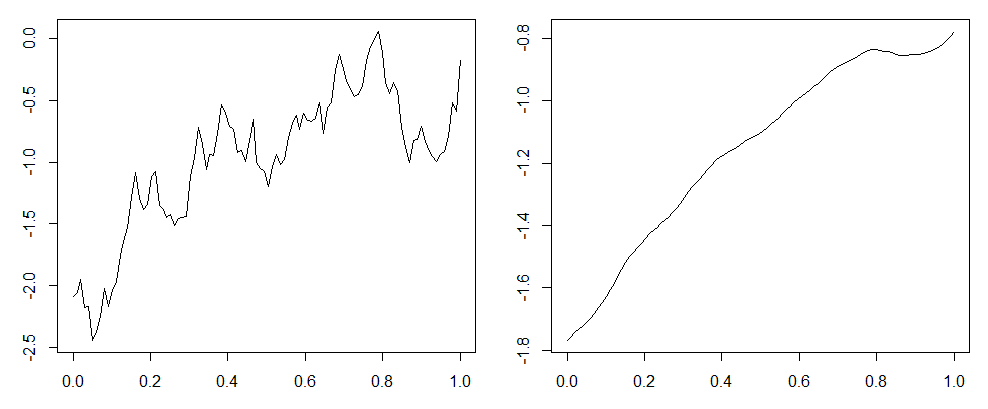
\includegraphics[width=1\textwidth]{mattplot.png}
\end{figure}



\item Problem 2
\item Problem 5
\end{enumerate}


\end{itemize}



\end{document}


